\section{Methodology}

\lstset{
  basicstyle=\small\ttfamily,
  captionpos=b,
  frame=single,
  breaklines=true,
  showstringspaces=false,
  aboveskip=2.5pt,
  belowskip=2pt
}

\subsection{Data collection and preprocessing}


\subsection{Model architecture}
A modellnek meg kell adni, hogy milyen dimenziójú bemenettel kell számolnia. Belátható, hogy a modellnek három rétege van, melyek teljesen összekapcsolt rétegek, amik alkotják a neurális hálózatot és a \verb|forward| függvényen keresztül halad át a bemeneti adatokon. Tegyük fel, hogy az \verb|input_dim| értéke 100, így annak 100 elemű vektorral kell rendelkeznie, ami az első réteget illeti.
\begin{lstlisting}[language=Python, caption={Modell Python kód tartalma}, label=modell]
    class TextClassifier(nn.Module):
        def __init__(self, input_dim):
            super(TextClassifier, self).__init__()
            self.fc1 = nn.Linear(input_dim, 64)
            self.fc2 = nn.Linear(64, 32)
            self.fc3 = nn.Linear(32, 2)

        def forward(self, x):
            x = torch.relu(self.fc1(x))
            x = torch.relu(self.fc2(x))
            x = self.fc3(x)
            return x
\end{lstlisting}
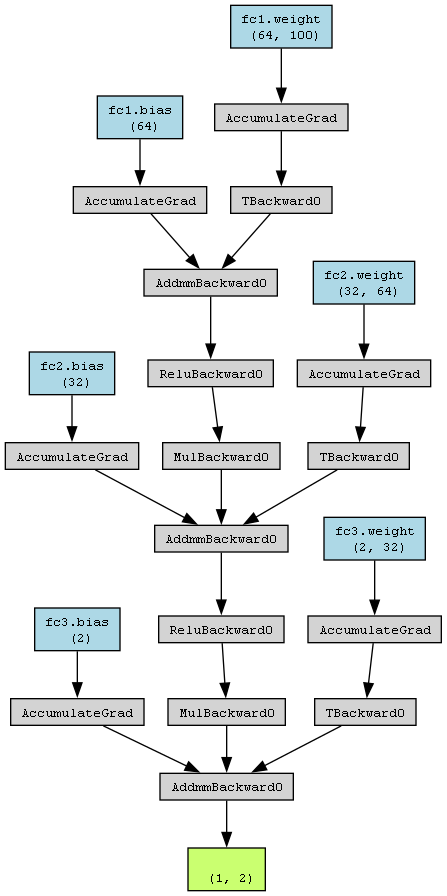
\includegraphics[width=0.4\textwidth]{text_classifier_model.png} \\